In diesem Abschnitt machen wir uns die getroffenen \nameref{ch:Content2:sec:a Posteriori} Annahmen 
zu Nutze. Nach dem Rendern von $Bild_{t}$ (und vor dem Rendern von $Bild_{t+1}$) nehmen wir die Sortierung
anhand der Pixelwerte von $Bild_{t}$ vor. 
\par
Bevor wir uns den Algorithmus anschauen muss jedoch geklärt werden, wieso wir hier an dieser Stelle 
überhaupt sortieren. Bisher haben wir uns alle möglichen Werte eines Pixels 
(in Gleichung \ref{eq:Pixel Schätzung Wahrscheinlichkeitsdichtefunktion}) angeschaut und daraus auf
eine Wahrscheinlichkeitsfunktion $H_{ij}(I)$ für die Werte eines Pixels geschlossen. 
Benutzen wir die inverse Funktion \ref{eq:inverse Funktion}, machen wir nichts Anderes, als 
zufällige Zahlen auf ein bestimmtes Wahrscheinlichkeitsquantil, das einer gewissen Sortierung entspricht,
abzubilden. Deshalb können wir die Pixelintensitäten innerhalb eines Blocks anhand ihrer 
Indizes (entspricht den Wahrscheinlichkeitsquantilen bei der Wahrscheinlichkeitsfunktion) 
sortieren! 

\begin{algorithm}[H]
    \caption{\textbf{Sortier Schritt t} nach dem Rendern von Frame t
    und vor dem Rendern von Frame t+1}
    \begin{algorithmic}[1]
        \State pixel \textbf{consists of} value,index;
        \State List framePixelsIntensities, noiseIntensities;
        \State $assert(sizeof(framePixelsIntensities)==BLOCKSIZE)$;
        \State $assert(sizeof(noiseIntensities)==BLOCKSIZE)$;
        \State List L $\leftarrow$ pixels of frame t in block;
        \State \hfill
        \State //init lists
        \State initList(framePixelsIntensities, pixelIntensity(L);
        \State $blueNoise_{t}$ = calcCorrectOffset(incomingbluenoisetexture);
        \State initList(noiseIntensities, pixelIntensity($blueNoise_{t}$));
        \State \hfill
        \State //sort the two lists by means of intensities
        \State sort(framePixelsIntensities);
        \State Sort(noiseIntensities);
        \State \hfill
        \State //now we reorder our seeds hence the sorted lists
        \For{$i = 1 .. BLOCKSIZE$}
        \State $sortedSeeds(noiseIntensities.getIndex(i)) = incomingSeeds(framePixelIntensities.getIndex(i))$;
        \EndFor
    \end{algorithmic}
    \label{alg:Sortier}
\end{algorithm}

Die Annahme der Lokalität, also der Homogenität einer Fläche innerhalb eines Blocks, 
erlaubt die Approximation des Histogramms \ref{fig:Pixelwerte} eines Pixels 
anhand der Intensitäten aller anderen Pixel innerhalb des Blocks.
Wird der Block zu groß gewählt, so wir die Approximation zu rechenintensiv die parallele Ausführbarkeit 
und die  Homogenitätseigenschaft gehen verloren, wohingegen 
zu kleine Blockgrößen nur eine sehr wage und ungenaue Approximation des 
Histogramms \ref{pic:histogramOfEstimates} liefern. Wir nehmen als Anzahl Pixel/BLOCK = 16
(nach \cite{hal02158423}),was eine gute Abwägung zwischen beiden Extrema liefert.
Dabei werden bei dem Algorithmus \ref{alg:Sortier} die Pixel anhand ihrer Intensitäten mitsamt 
ihrer Anfangswerte als Indices sortiert. Dies kann man, wie anfangs erwähnt, als Zuordnung 
von zufälligen Zahlen (Anfangswerte) zu ihren Quantilen (Intensitätenintervalle) des Histogramms deuten.
Eine \nameref{ch:Content1:sec:blue noise} Zahlenfolge wird ebenfalls mitsamt ihren Indices sortiert.
An der Stelle der niedrigsten \nameref{ch:Content1:sec:blue noise}-Intensität wird der Anfangswert abgespeichert,
der für die niedrigste Intensität des Bildes zuständig war etc. 
\newpage
Nehmen wir hier nun die im vorherigen Abschnitt \ref{ch:Content2:sec:a Posteriori} postulierte Behauptung 
auf, 

\begin{itemize}
    \item[\uproman{1}.)] dass der Farbwert eines Pixels und Wahl des Anfangswertes(siehe Gleichung 
                        \ref{eq:inverse Funktion}) gleichbedeutend sind und 
    \item[\uproman{2}.)] die Ähnlichkeit von $Bild_{t}$ und $Bild_{t+1}$(bzw. Statik der Szene)
\end{itemize}

in betracht ziehen, sind die Pixel von $Bild_{t+1}$ folglich \nameref{ch:Content1:sec:blue noise} 
verteilt. 

\par

Hierbei muss noch eine wichtige Anmerkung gemacht werden. Die Fehlerverteilung
der Pixelwerte im Bildraum konvergiert auf diese Weise nicht zu einer 
blue noise Verteilung, denn wir wechseln in jedem Bild die 
verwendeten blue noise Texturen(theoretisch, praktischerweise werden wir hier eine
Textur verwenden und mit Erkenntnissen aus \nameref{ch:Content1:sec:Quasi-Zufallsfolgen}) 
quasi-zufällig zugreifen um so einen solchen Effekt zu erreichen). 
Dieser Schritt alleine reicht also nicht für den erwünschten Effekt zu erreichen.

\label{subsec:Blockgröße}
\subsubsection{Blockgöße}

\newpage

\begin{figure}[H]

    \begin{subfigure}{\textwidth}
        \centering 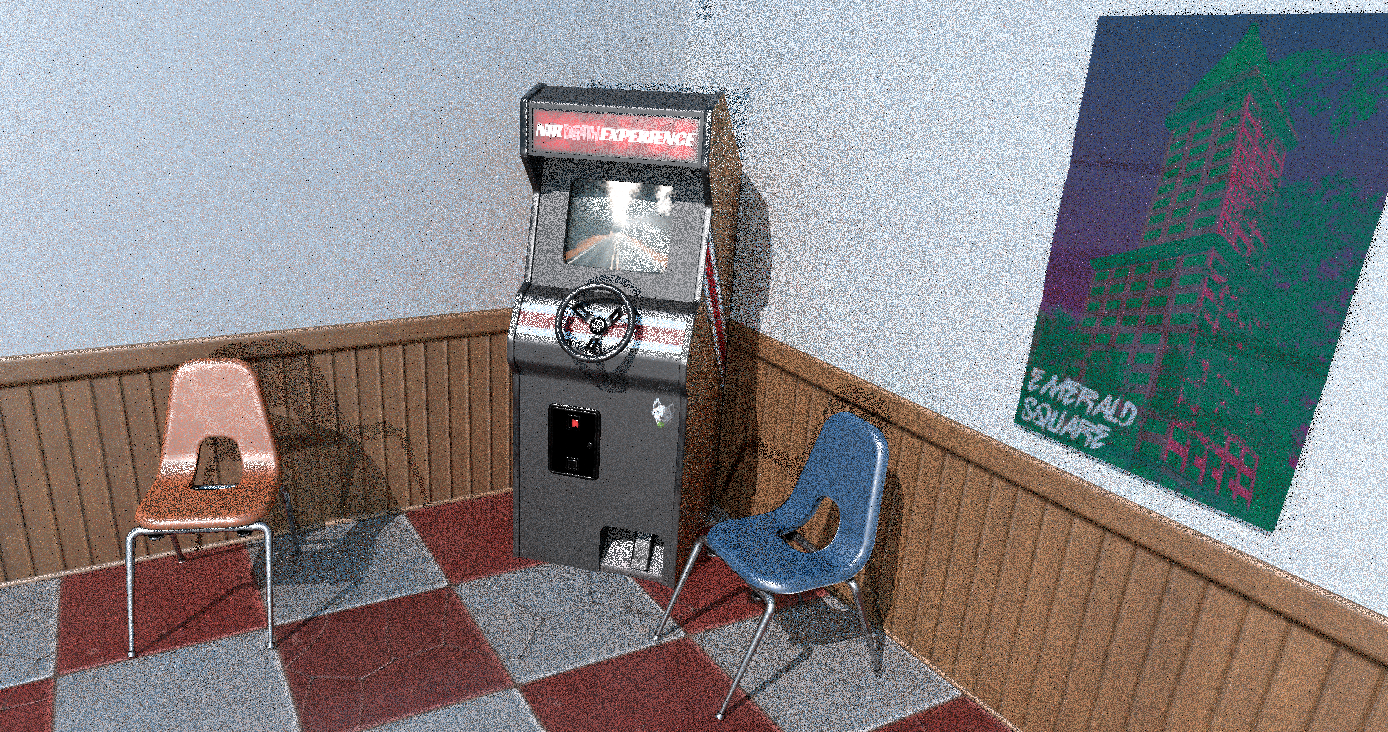
\includegraphics[scale=.25]{content/TemporalerAlg/Bilder/Sorting/Screenshots/seed_debug_3.0_selection.png}
        \caption{Szene}
        \label{fig:Nur_Sorting_Szene_t1}
    \end{subfigure}
    \begin{subfigure}{0.5\textwidth}
        \centering 
\includegraphics[width=0.4\linewidth]{content/TemporalerAlg/Bilder/Sorting/Screenshots/seed_debug_3.0_ausschnitt.png} 
        \caption{Szenenausschnitt}
        \label{fig:Nur_Sorting_ausschnitt_t1}
    \end{subfigure}
    \begin{subfigure}{0.5\textwidth}
        \centering 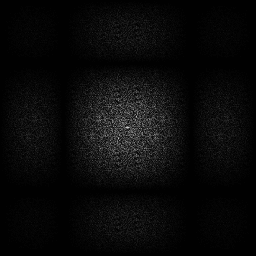
\includegraphics[width=0.4\linewidth]{content/TemporalerAlg/Bilder/Sorting/Screenshots/Spektren/seed_debug_3.0_ausschnitt.png}
        \caption{Fouriertransformierte des Ausschnitts}
        \label{fig:Nur_Sorting_Fouriertransformierte_t1}
    \end{subfigure}
        \caption{Zeitpunkt t=1}
        \label{fig:Nur_Sorting_Verlauf_t1}
\end{figure}

\begin{figure}[H]
    \begin{subfigure}{\textwidth}
        \centering 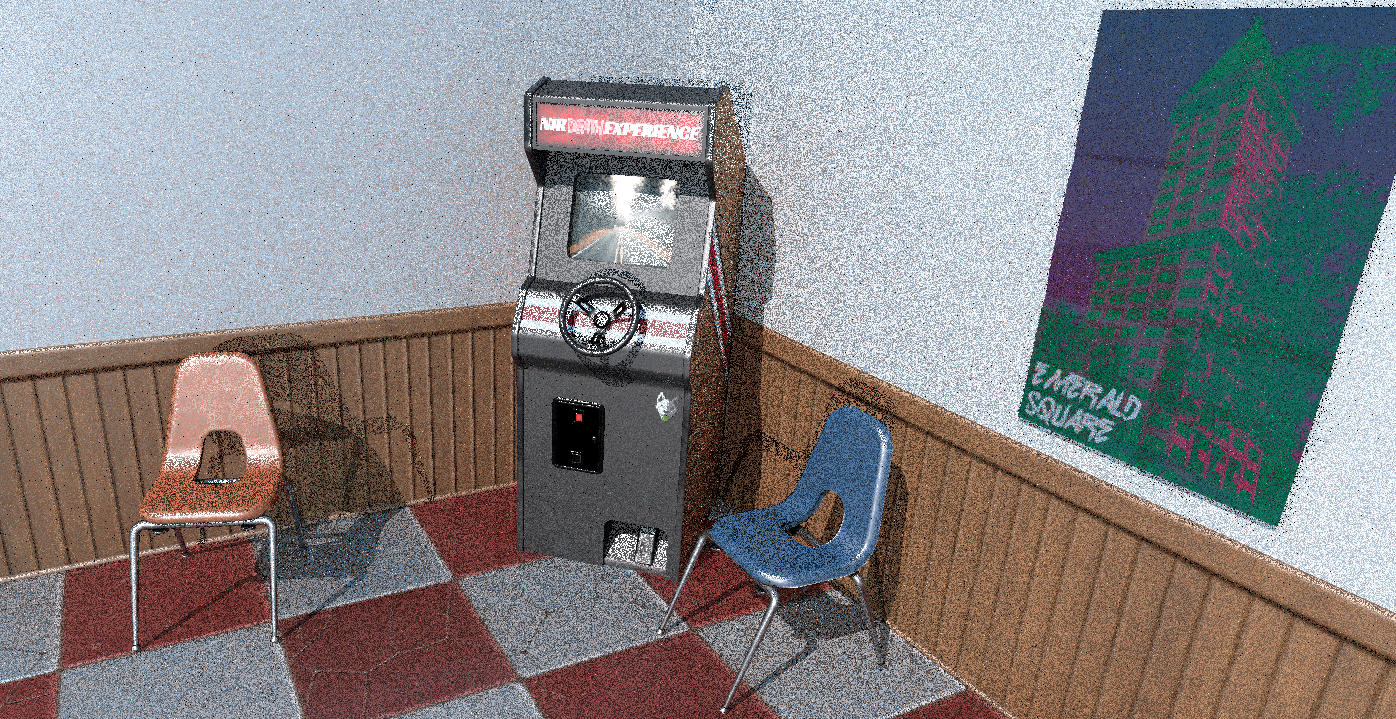
\includegraphics[scale=.25]{content/TemporalerAlg/Bilder/Sorting/Screenshots/seed_debug_4.0_selection.png}
        \caption{Szene}
        \label{fig:Nur_Sorting_Szene_t2}
    \end{subfigure}
    \begin{subfigure}{0.5\textwidth}
        \centering
\includegraphics[width=0.4\linewidth]{content/TemporalerAlg/Bilder/Sorting/Screenshots/seed_debug_4.0_ausschnitt.png} 
        \caption{Szenenausschnitt}
        \label{fig:Nur_Sorting_ausschnitt_t2}
    \end{subfigure}
    \begin{subfigure}{0.5\textwidth}
        \centering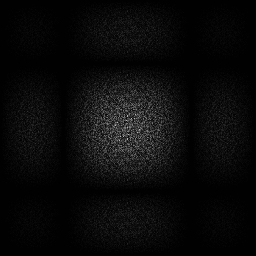
\includegraphics[width=0.4\linewidth]{content/TemporalerAlg/Bilder/Sorting/Screenshots/Spektren/seed_debug_4.0_ausschnitt.png}
        \caption{Fouriertransformierte des Ausschnitts}
        \label{fig:Nur_Sorting_Fouriertransformierte_t2}
    \end{subfigure}
        \caption{Zeitpunkt t=2}
        \label{fig:Nur_Sorting_Verlauf_t2}
\end{figure}

\begin{figure}[H]
    \begin{subfigure}{\textwidth}
        \centering 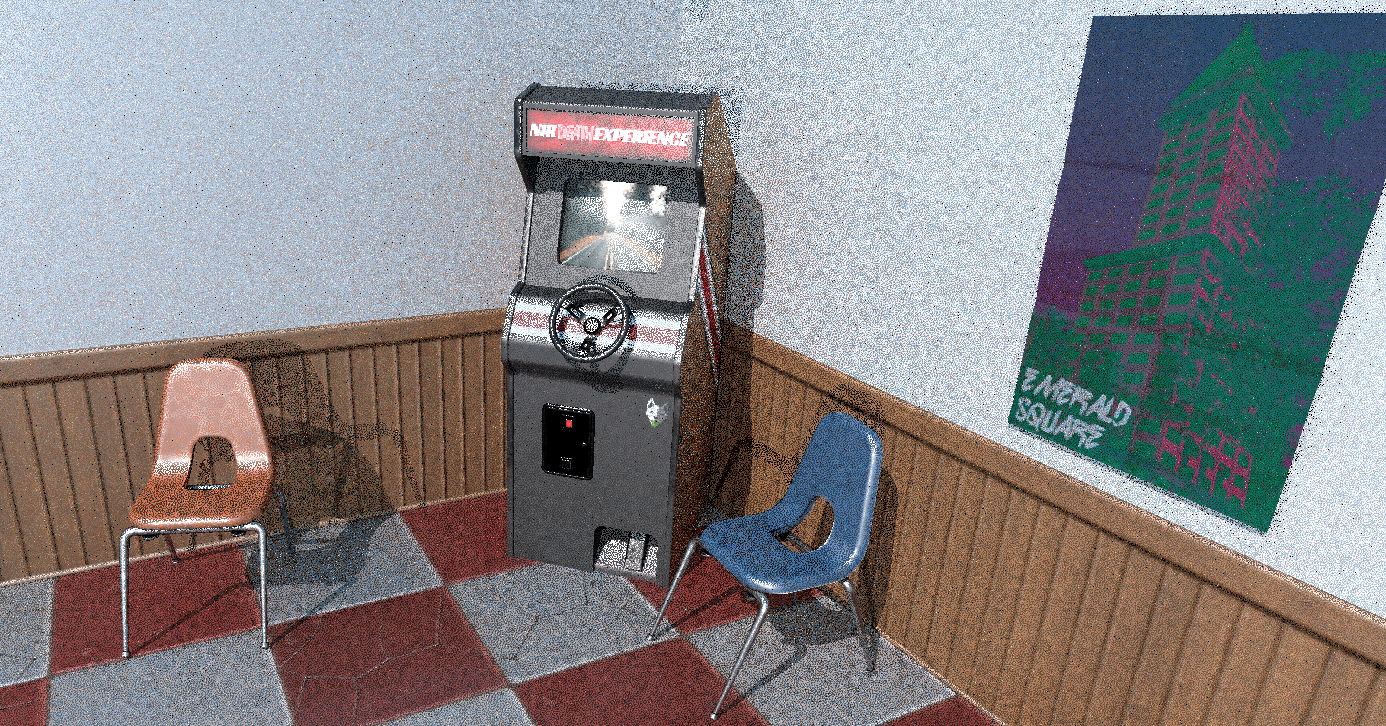
\includegraphics[scale=.25]{content/TemporalerAlg/Bilder/Sorting/Screenshots/seed_debug_5.0_selection.png}
        \caption{Szene}
        \label{fig:Nur_Sorting_Szene_t3}
    \end{subfigure}
    \begin{subfigure}{0.5\textwidth}
        \centering
\includegraphics[width=0.4\linewidth]{content/TemporalerAlg/Bilder/Sorting/Screenshots/seed_debug_5.0_ausschnitt.png} 
        \caption{Szenenausschnitt}
        \label{fig:Nur_Sorting_ausschnitt_t3}
    \end{subfigure}
    \begin{subfigure}{0.5\textwidth}
        \centering
\includegraphics[width=0.4\linewidth]{content/TemporalerAlg/Bilder/Sorting/Screenshots/Spektren/seed_debug_5.0_ausschnitt.png}
        \caption{Fouriertransformierte des Ausschnitts}
        \label{fig:Nur_Sorting_Fouriertransformierte_t3}
    \end{subfigure}
        \caption{Zeitpunkt t=3}
        \label{fig:Nur_Sorting_Verlauf_t3}
\end{figure}

\begin{figure}[H]
    \begin{subfigure}{\textwidth}  
        \centering 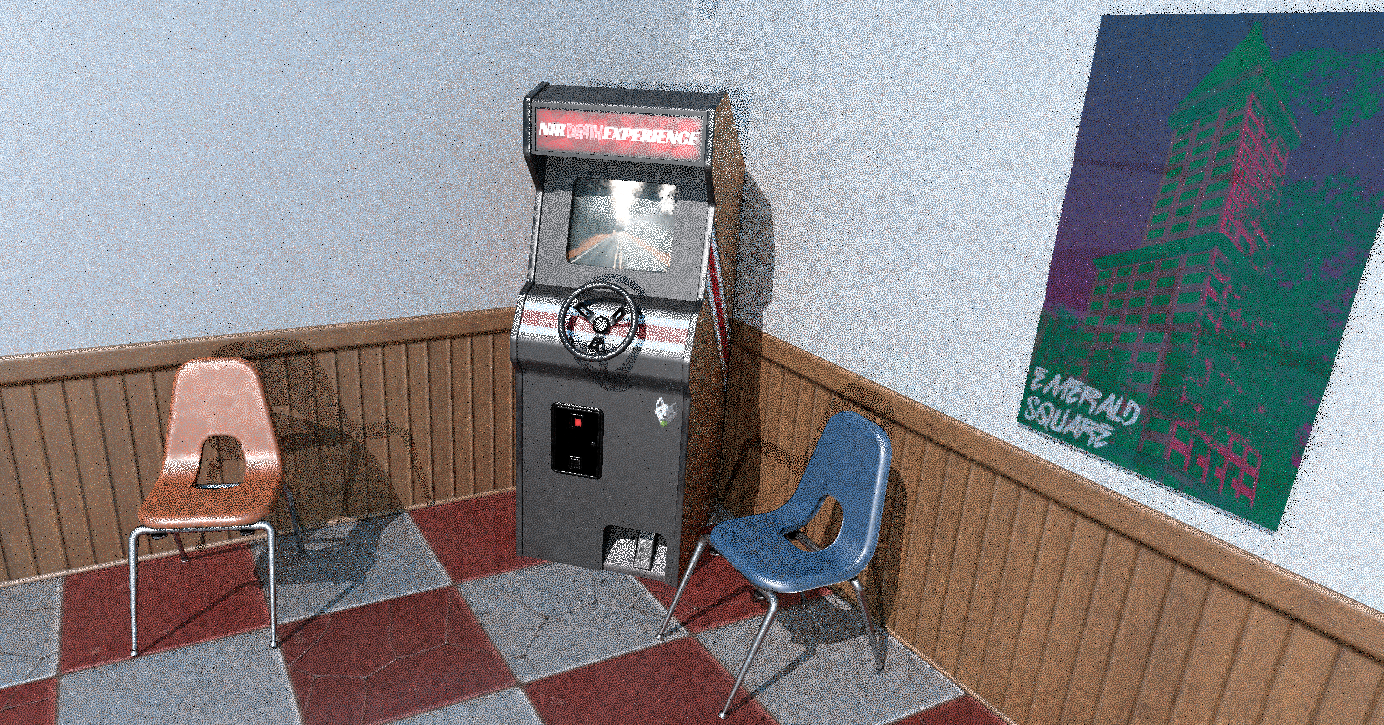
\includegraphics[scale=.25]{content/TemporalerAlg/Bilder/Sorting/Screenshots/seed_debug_6.0_selection.png}
        \caption{Szene}
        \label{fig:Nur_Sorting_Szene_t4}
    \end{subfigure}
    \begin{subfigure}{0.5\textwidth}
        \centering
\includegraphics[width=0.4\linewidth]{content/TemporalerAlg/Bilder/Sorting/Screenshots/seed_debug_6.0_ausschnitt.png} 
        \caption{Szenenausschnitt}
        \label{fig:Nur_Sorting_ausschnitt_t4}
    \end{subfigure}
    \begin{subfigure}{0.5\textwidth}
        \centering
\includegraphics[width=0.4\linewidth]{content/TemporalerAlg/Bilder/Sorting/Screenshots/Spektren/seed_debug_6.0_ausschnitt.png}
        \caption{Fouriertransformierte des Ausschnitts}
        \label{fig:Nur_Sorting_Fouriertransformierte_t4}
    \end{subfigure}
        \caption{Zeitpunkt t=4}
        \label{fig:Nur_Sorting_Verlauf_t4}
\end{figure}

\begin{figure}[H]
    \begin{subfigure}{\textwidth}   
        \centering 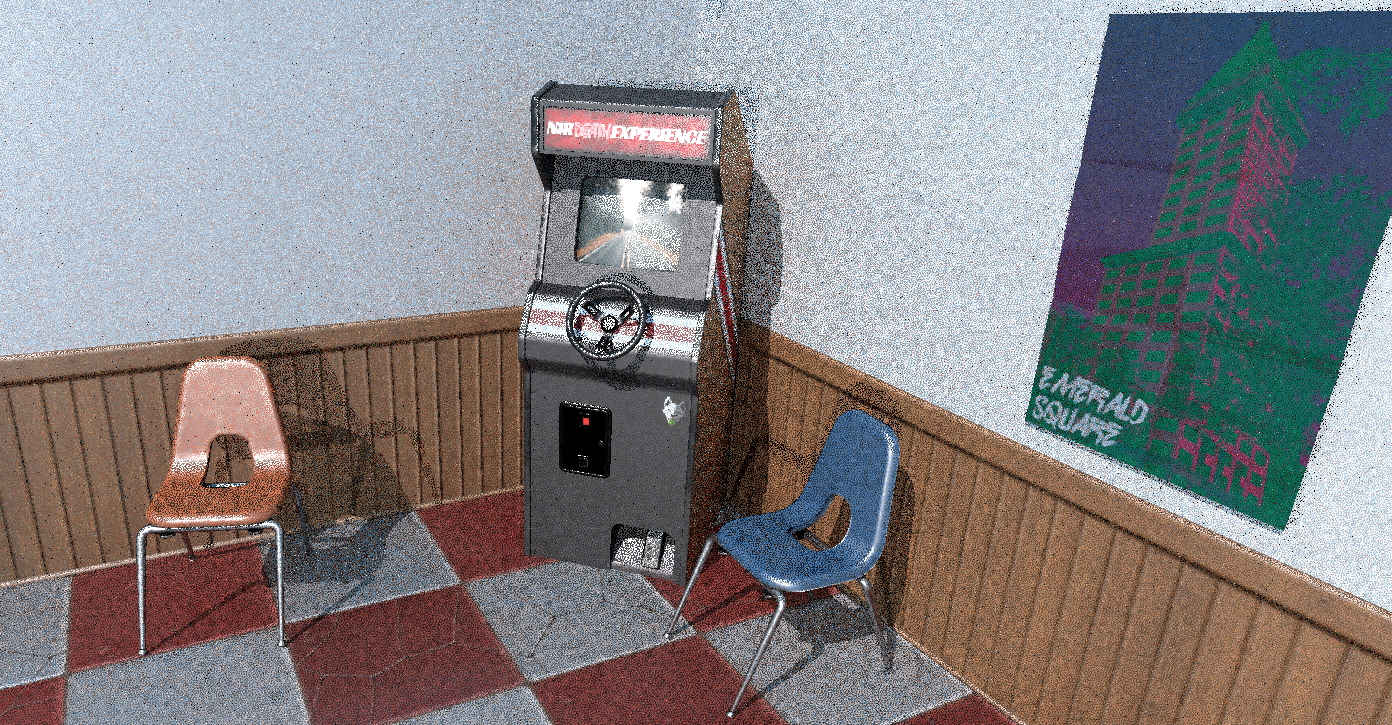
\includegraphics[scale=.25]{content/TemporalerAlg/Bilder/Sorting/Screenshots/seed_debug_7.0_selection.png}
        \caption{Szene}
        \label{fig:Nur_Sorting_Szene_t5}
    \end{subfigure}
    \begin{subfigure}{0.5\textwidth}
        \centering
\includegraphics[width=0.4\linewidth]{content/TemporalerAlg/Bilder/Sorting/Screenshots/seed_debug_7.0_ausschnitt.png} 
        \caption{Szenenausschnitt}
        \label{fig:Nur_Sorting_ausschnitt_t5}
    \end{subfigure}
    \begin{subfigure}{0.5\textwidth}
        \centering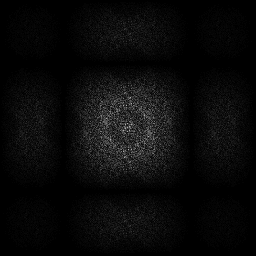
\includegraphics[width=0.4\linewidth]{content/TemporalerAlg/Bilder/Sorting/Screenshots/Spektren/seed_debug_7.0_ausschnitt.png}
        \caption{Fouriertransformierte des Ausschnitts}
        \label{fig:Nur_Sorting_Fouriertransformierte_t5}
    \end{subfigure}
        \caption{Zeitpunkt t=5}
        \label{fig:Nur_Sorting_Verlauf_t5}
\end{figure}

\begin{figure}[H]
    \begin{subfigure}{\textwidth}   
        \centering 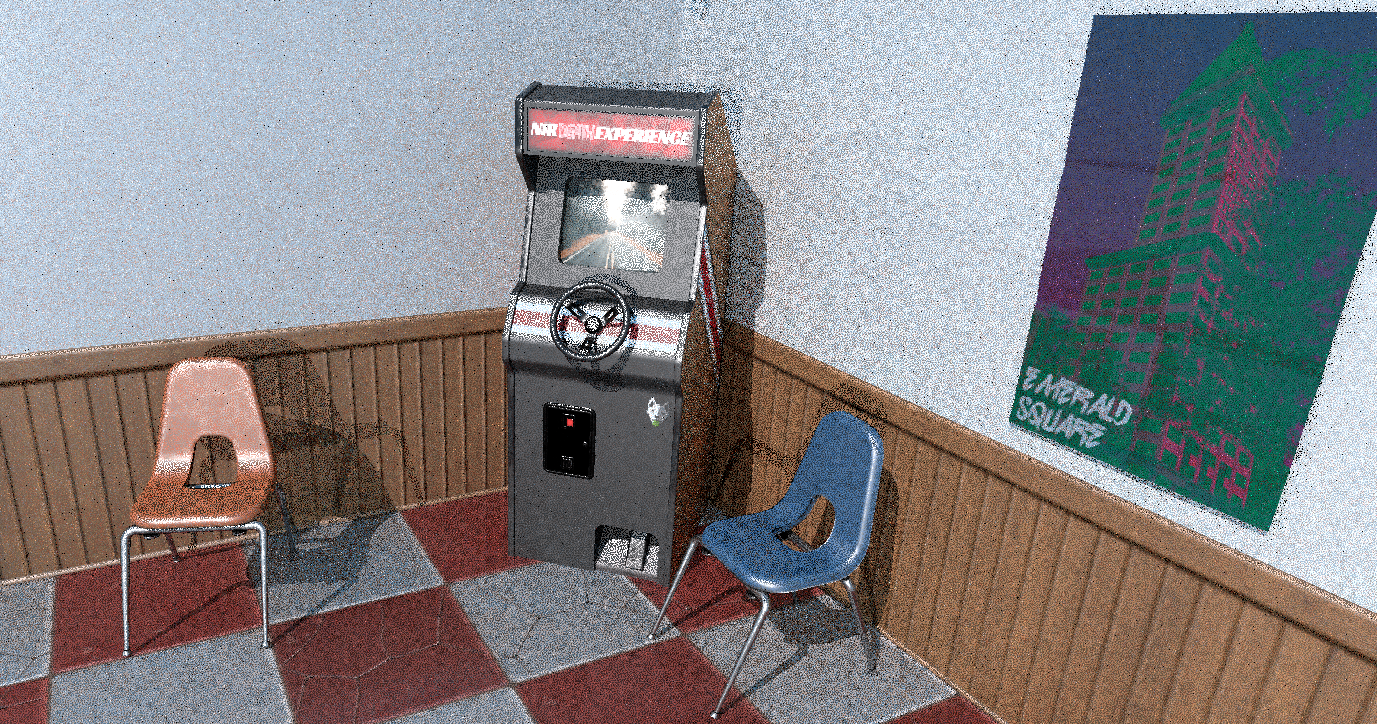
\includegraphics[scale=.25]{content/TemporalerAlg/Bilder/Sorting/Screenshots/seed_debug_8.0_selection.png}
        \caption{Szene}
        \label{fig:Nur_Sorting_Szene_t6}
    \end{subfigure}
    \begin{subfigure}{0.5\textwidth}
        \centering
\includegraphics[width=0.4\linewidth]{content/TemporalerAlg/Bilder/Sorting/Screenshots/seed_debug_8.0_ausschnitt.png} 
        \caption{Szenenausschnitt}
        \label{fig:Nur_Sorting_ausschnitt_t6}
    \end{subfigure}
    \begin{subfigure}{0.5\textwidth}
        \centering
\includegraphics[width=0.4\linewidth]{content/TemporalerAlg/Bilder/Sorting/Screenshots/Spektren/seed_debug_8.0_ausschnitt.png}
        \caption{Fouriertransformierte des Ausschnitts}
        \label{fig:Nur_Sorting_Fouriertransformierte_t6}
    \end{subfigure}
        \caption{Zeitpunkt t=5}
        \label{fig:Nur_Sorting_Verlauf_t6}
\end{figure}

\begin{figure}[H]
    \begin{subfigure}{\textwidth}   
        \centering 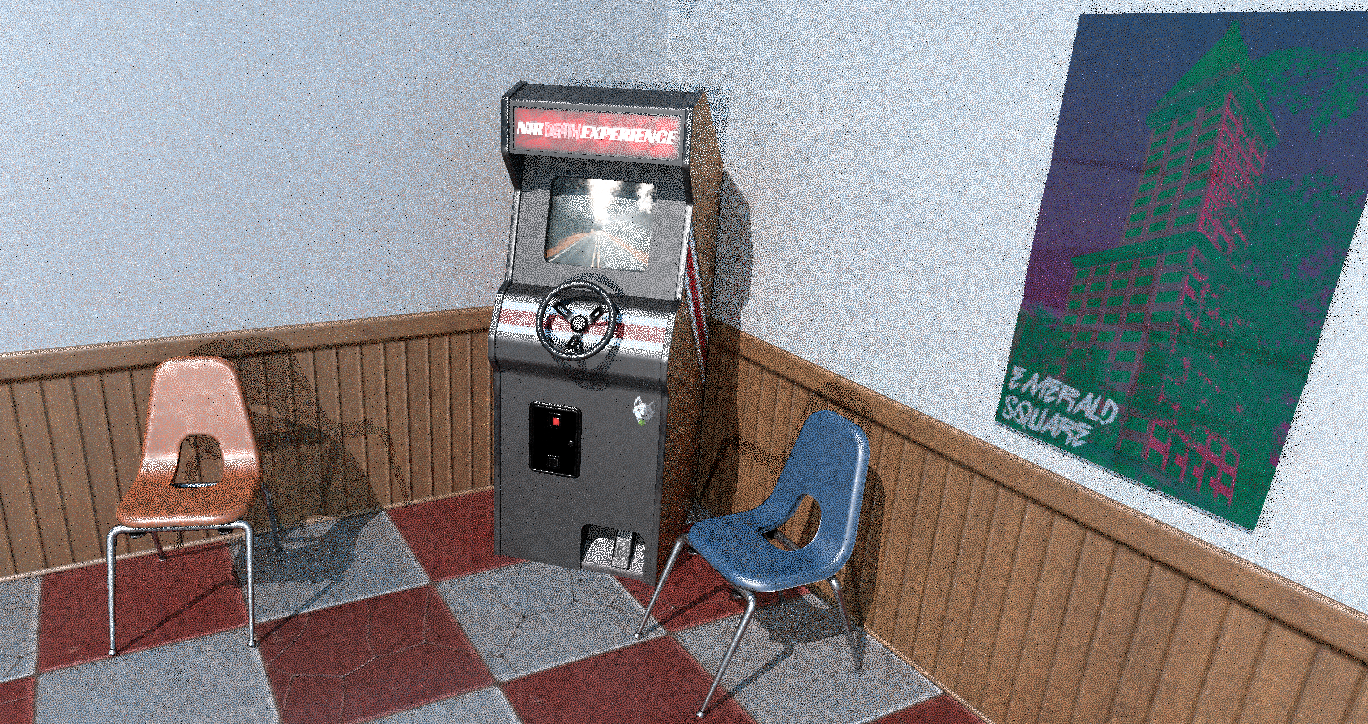
\includegraphics[scale=.25]{content/TemporalerAlg/Bilder/Sorting/Screenshots/seed_debug_9.0_selection.png}
        \caption{Szene}
        \label{fig:Nur_Sorting_Szene_t7}
    \end{subfigure}
    \begin{subfigure}{0.5\textwidth}
        \centering
\includegraphics[width=0.4\linewidth]{content/TemporalerAlg/Bilder/Sorting/Screenshots/seed_debug_9.0_ausschnitt.png} 
        \caption{Szenenausschnitt}
        \label{fig:Nur_Sorting_ausschnitt_t7}
    \end{subfigure}
    \begin{subfigure}{0.5\textwidth}
        \centering
\includegraphics[width=0.4\linewidth]{content/TemporalerAlg/Bilder/Sorting/Screenshots/Spektren/seed_debug_9.0_ausschnitt.png}
        \caption{Fouriertransformierte des Ausschnitts}
        \label{fig:Nur_Sorting_Fouriertransformierte_t7}
    \end{subfigure}
        \caption{Zeitpunkt t=5}
        \label{fig:Nur_Sorting_Verlauf_t7}
\end{figure}